\section{Data Model}
\label{sec:model}

We propose that vertices and edges, rather than whole graphs, serve as
units of temporal history.  We now describe the {\em logical}
representation of an evolving graph, called a \tg.  A \tg represents a
single graph, and models evolution of its topology and of vertex and
edge attributes.  \eat{Figure~\ref{fig:tg_ve} gives an example of a
  \tg that shows evolution of a co-authorship network.}

Following the SQL:2011
standard~\cite{DBLP:journals/sigmod/KulkarniM12}, a period (or
interval) $\bp = [s, e)$ represents a discrete set of time instances,
  starting from and including the start time $s$, continuing to but
  excluding the end time $e$.  Time instances contained within the
  period have limited precision, and the time domain has total order.
  In the rest of this paper we use the terms interval and timestamp
  interchangeably.

\eat{
\begin{figure}[t!]
\centering
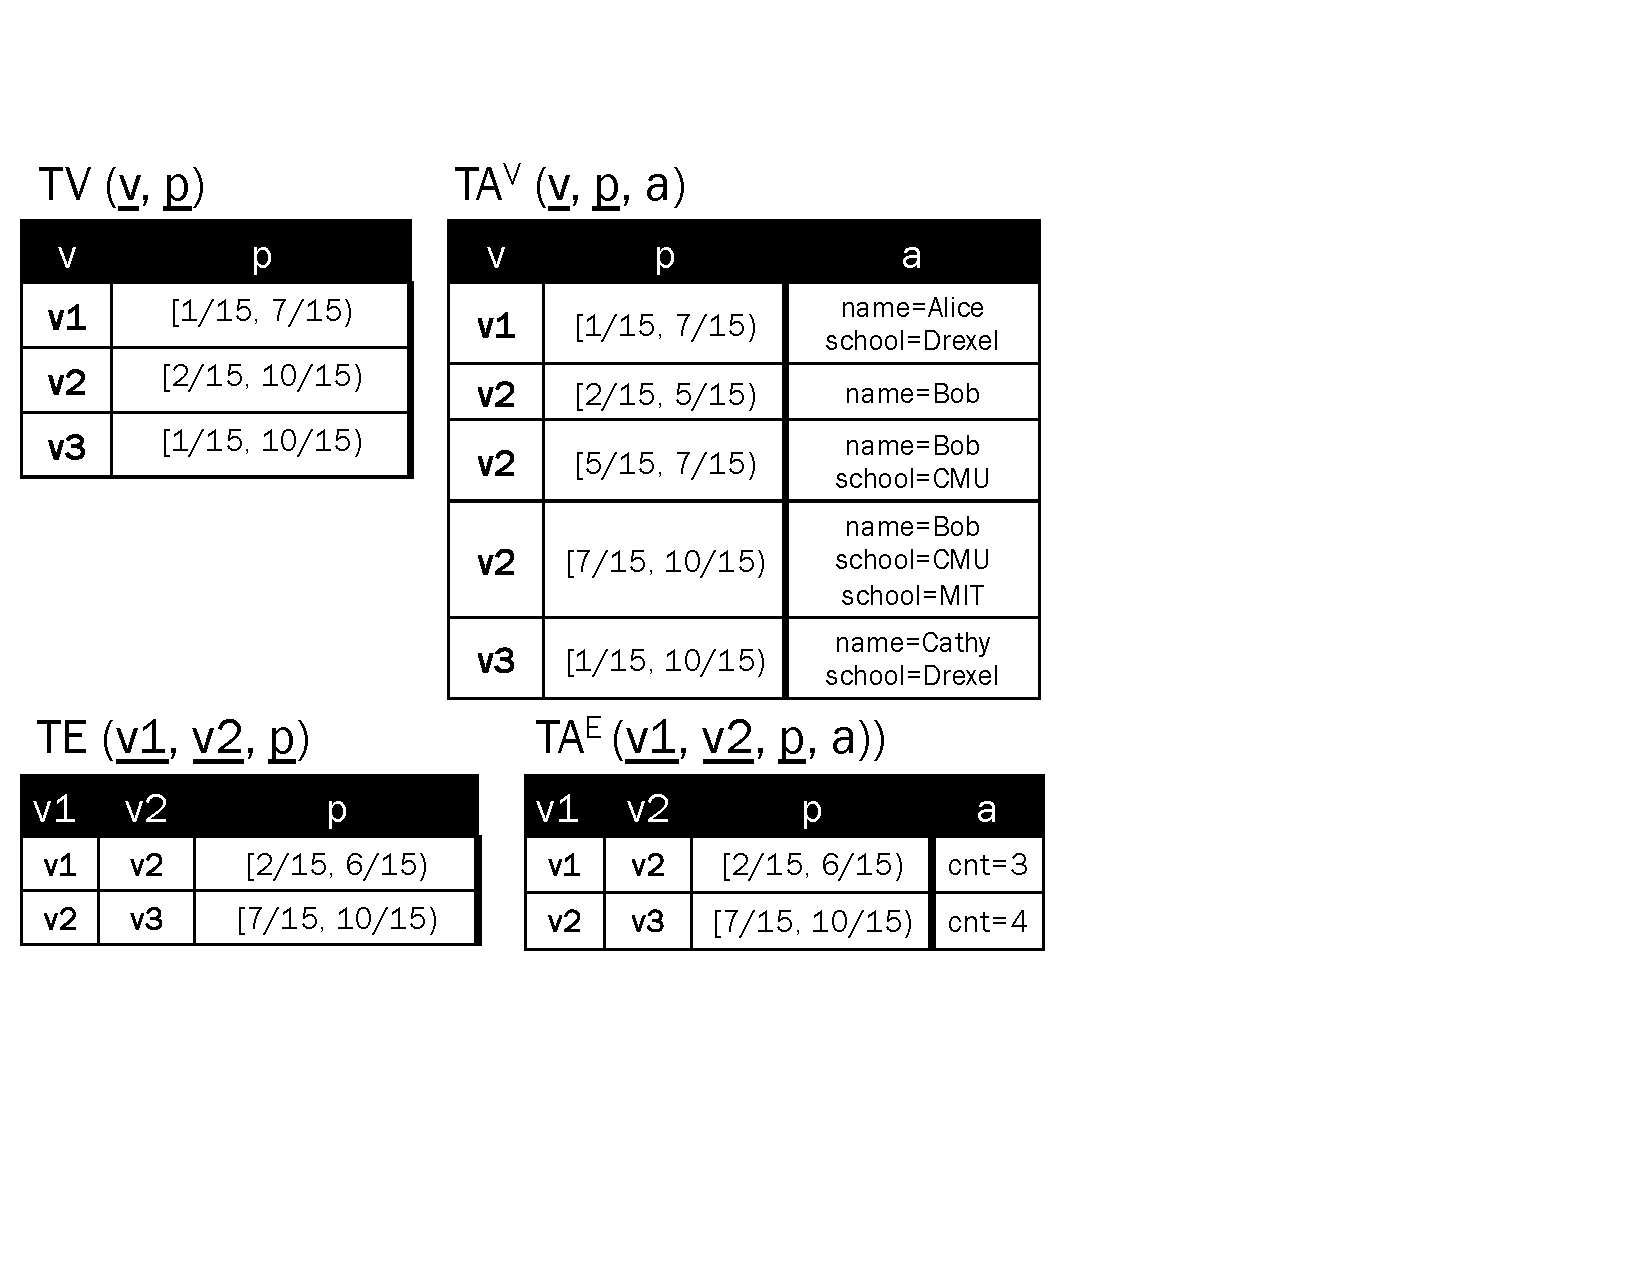
\includegraphics[width=3in]{figs/T1_rel.pdf}
%\vspace{-0.5cm}
\caption{\tg \insql{T1}.}
\vspace{-0.5cm}
\label{fig:tg_ve}
\end{figure}
}

A \tg is represented with four temporal SQL
relations~\cite{DBLP:conf/vldb/BohlenSS96}, and uses sequence
semantics~\cite{Dignos2012}, associating a fact (existence of a vertex
or edge, and an assignment of a value to a vertex or edge attribute)
with an interval.

A snapshot of a temporal relation $R$, denoted $\tau_c(R)$ is the
state of $R$ at time point $c$.

We use the property graph model~\cite{GraphDB} to represent vertex and
edge attributes: each vertex and edge during period $\bp$ is
associated with a (possibly empty) {\em set} of properties, and each
property is represented by a key-value pair.  Property values are not
restricted to be of atomic types, and may, e.g., be sets, maps or
tuples.

We now give a formal definition of a \tg.

\begin{definition}[TGraph]
A \tg is a pair $\tve=(\tv, \te)$. \tv is a valid-time temporal SQL
relation with schema $\tv(\underline{v}, \underline{\bp})$ that
associates a vertex with the time period during which it is
present. \te is a valid-time temporal SQL relation with schema
$\te(\underline{v_1}, \underline{v_2}, \underline{\bp})$, connecting
pairs of vertices from \tv.  
%
\tve optionally includes vertex and edge attribute relations
$\tav(\underline{v}, \underline{\bp}, a)$ and $\tae(\underline{v_1},
\underline{v_2}, \underline{\bp}, a)$, where $a$ is a nested attribute
consisting of key-value property pairs.
%
Relations of \tve must meet the following requirements:

\begin{description}[noitemsep]
\item [R1: Unique vertices/ edges] In every snapshot $\tau^s_c (\tav)$
  and $\tau^s_c (\tae)$ a vertex/edge exists at most once.
\item [R2: Unique attribute values] In every snapshot $\tau^s_c
  (\tav)$ and $\tau^s_c (\tae)$, a vertex/edge is associated with at
  most one attribute (which is itself a set of key-value pairs
  representing properties).
\item [R3: Referential integrity] In every snapshot $\tau^s_c (\tve)$,
  foreign key constraints hold from $\tau^s_c (\te)$ (on both $v_1$
  and $v_2$) and $\tau^s_c (\tav)$ to $\tau^s_c (\tv)$, and from
  $\tau^s_c (\tae)$ to $\tau^s_c (\te)$.
\end{description}
\label{def:tg}
\vspace{-0.5cm}
\end{definition}

Requirements {\bf R1, R2, R3} guarantee soundness of the \tg data
structure, ensuring that every snapshot of a \tg is a valid graph.
 
\eat{\tv and \te are temporally coalesced:
\vspace{-0.3cm}
\begin{multline}
\vspace{-0.3cm}
\forall \tv(v, \bp)~~\nexists \tv(v, \bq)~~| \\
                       \pred{\bp}{meets}{\bq'}~\lor~\pred{\bp}{contains}{\bq}~\lor~\pred{\bp}{overlaps}{\bq}
\label{def:tg:c2}
\end{multline}
\vspace{-0.7cm}
\begin{multline}
\forall \te(v_1, v_2, \bp)~~\nexists \te(v_1,v_2, \bq)~~| \\
                       \pred{\bp}{meets}{\bq}~\lor~\pred{\bp}{contains}{\bq}~\lor~\pred{\bp}{overlaps}{\bq}
\label{def:tg:c3}
\end{multline}
}

\eat{An edge connects a pair of vertices that exist at the time when the edge exists:
\vspace{-0.3cm}
\begin{multline}
\forall \te(v_1, v_2, \bp)~~\exists \tv(v_1, \bp_1), \tv(v_2, \bp_2)~~| \\
                       \pred{\bp_1}{contains}{\bp}~\wedge~\pred{\bp_2}{contains}{\bp}
\label{def:tg:c1}
\end{multline}
\vspace{-0.5cm}
}

\eat{\tve optionally includes vertex and edge attribute relations \tav
and \tae.  Both are coalesced, and associate sets of properties with
existing vertices and edges.}

\eat{\vspace{-0.3cm}
\begin{multline}
\forall \tav(v, p, a)~~\nexists \tav(v, p', a')~~| \\
                       \pred{p}{meets}{p'}~\lor~\pred{p}{contains}{p'}~\lor~\pred{p}{overlaps}{p'}
\label{def:tg:c4}
\end{multline}
\vspace{-0.5cm}
\begin{multline}
\forall \tav(v, p, a)~~\exists \tv(v,p')~~|~~\pred{p'}{contains}{p}
\label{def:tg:c5}
\end{multline}
\vspace{-0.5cm}
\begin{multline}
\forall \tae(v_1, v_2, p, a)~~\nexists \tae(v_1, v_2, p', a')~~| \\
                       \pred{p}{meets}{p'}~\lor~\pred{p}{contains}{p'}~\lor~\pred{p}{overlaps}{p'}
\label{def:tg:c6}
\end{multline}
\vspace{-0.5cm}
\begin{multline}
\forall \tae(v_1, v_2, p, a)~~\exists \te(v_1,v_2,p')~~|~~\pred{p'}{contains}{p}
\label{def:tg:c7}
\end{multline}
\vspace{-0.6cm}
\label{def:tg}
\end{definition}
\vspace{-0.3cm}
}

Graphs may be directed or undirected.  For undirected graphs we choose
a canonical representation of an edge, with $v_1 \leq v_2$ (self-loops
are allowed).  Because we use the source and destination vertex id
pair as the identifier for the edges, at most two edges can exist
between any two vertices (one in each direction) at any time point.
That is, we do not support multigraphs.

\eat{Conditions~\ref{def:tg:c2},~\ref{def:tg:c3},~\ref{def:tg:c4},
  and~\ref{def:tg:c6} in Definition~\ref{def:tg} state that all
  relations of \tve are coalesced~\cite{DBLP:conf/vldb/BohlenSS96} ---
  each fact (existence of a vertex or edge, or an assignment of a
  value to a vertex or edge attribute) is represented exactly once for
  each time period of maximal length during which it holds. } 

\eat{ For point-stamped temporal models, requiring that relations be
  coalesced avoids semantic ambiguity
  (see~\cite{DBLP:reference/db/JensenS09k} Fig. 2 and its
  description).}

\eat{It is not required that a vertex or an edge be represented in
  \tav and \tae --- a vertex or edge that never had any associated
  properties will have no corresponding tuples in \tav or \tae.}

\eat{ Condition~\ref{def:tg:c1} in Definition~\ref{def:tg} states the
  natural integrity constraint that an edge linking two vertices can
  only exist during a time when both vertices exist. Here,
  $\pred{p}{contains}{q}$ is the Allen \predName{contains} relation
  with equality~\cite{allen83}, defined as $\bp.start \leq \bq.start
  \wedge \bp.end \geq \bq.end$.  Consider the vertex-edge representation
  of \tg \insql{T1} in Figure~\ref{fig:tg_ve}, where edge $e(v_1,v_2)$
  exists during the entire period when both $v_1$ and $v_2$ exist,
  while edge $e(v_2,v_3)$ exists only for a portion of the period when
  both $v_2$ and $v_3$ exist.}

In the \tg representation of Definition~\ref{def:tg}, vertex and edges
attributes are stored as collections of properties.  That said,
Definition~\ref{def:tg} presents a {\em logical} data structure that
admits different physical representations, including, e.g., a columnar
representation (each property in a separate relation, supporting
different change rates), by a hash-based representation
of~\cite{DBLP:conf/sigmod/SunFSKHX15}, or in some other way.  Since
our focus is on distributed computation over very large evolving
graphs, we do not assume that the data is stored in a relational
database.  This logical model allows for distributed storage in HDFS
and many other variants.

\eat{We
  leave an experimental comparison of different physical
  representations of vertex and edge attributes to future work.}

\eat{
Definition~\ref{def:tg} gives a columnar representation of vertex and
edge attributes.  Such a representation naturally supports {\em schema
  evolution} and can lead to more efficient physical representations,
especially when values of different attributes change at different
rates.  That said, our support of non-atomic types allows to combine
multiple, or even all, vertex (resp. edge) attributes in a single
attribute relation, as is the case in \tav Figure~\ref{fig:tg_ve}.}

\eat{Our choice to use attribute relations is in contrast to
  representing vertex and edge attributes as part of \tv and \te.  The
  main reason is to streamline the enforcement of referential
  integrity constraints of Definition~\ref{def:tg}.}  \eat{Consider
  again the example in Figure~\ref{fig:tg_ve}.  If vertex attributes
  were stored as part of \tv, then there would be two tuples for $v_2$
  in this relation whose validity periods overlap with that of edge
  $e(v_1, v_2)$ --- one for each $[2/15, 5/15)$ and $[5/15, 7/15)$.
      This would in turn require that $e(v_1, v_2)$ be mapped to two
      tuples in \tv as part of referential integrity checking on
      $v_2$.  Matching a tuple with a set of tuples in the referenced
      table, while supported by the SQL:2011 standard, is potentially
      inefficient, and we avoid it in our representation.}
%
\eat{Another reason for storing \tav and \tae separately is that in many
cases we are interested in applying operations (e.g., analytics) only
to graph topology, and in that case \tv and \te are sufficient.}
%

\eat{
\trg and \tve are equivalent in terms of the information they contain.
\trg can be computed from \tve by (1) enumerating all time points
during which some change occurred, i.e., those that appear as either
the start or the end of some time period in \tv, \te, \tav, and \tae;
(2) computing \trg periods by generating pairs of adjacent time points
from step 1, and sorting them by $start$; (3) constructing a graph $g$
for each time period $\bp$ by selecting tuples from \tv, \te, \tav, and
\tae that overlap with $\bp$.
}

\eat{
To compute \tve from \trg, we iterate over $\trg (g,p)$, computing
$\tv_g(v,p)$ (similarly for $\te_g$, $\tav_g$, $\tav_g$) for each
tuple, collecting $\tv_g \rightarrow \tv$, $\te_g \rightarrow \te$,
$\tav_g \rightarrow \tav$, $\tae_g \rightarrow \tae$, and coalescing
each \tv, \te, \tav, \tae.
}


